\section{Experiment P2B: uniform all-pairs ranging-rate sweep}
\subsection{Purpose and matched protocol}
P2B asks how much of the P2A localization improvement remains when all six available pairwise UWB links are activated less often. The comparison fixes the four trajectories, \SI{60}{s} duration, \SI{100}{Hz} inertial sampling, 20 stochastic seeds, noise and bias parameters, known initial poses, perturbed initial velocities, and joint EKF. Within each seed, all rates use exactly the same noisy IMU signals, initial perturbation, and pre-generated range values. Only the ranging activation schedule changes. Thus each row of the rate comparison has an identical underlying motion and stochastic realization.

At positive rate \(f\), all six undirected pairs exchange ranges every \(1/f\) seconds, beginning after initialization and ending at \SI{60}{s}. The scheduling times are nested within the maximum \SI{10}{Hz} schedule. Let \(C\) count individual pairwise range exchanges; then \(\rho_{\mathrm{comm}}=C/3600\) relative to the P2A full-communication reference. Table~\ref{tab:p2b_schedule} gives the exact cost of every condition. The endpoint conditions at 0 and \SI{10}{Hz} reproduce the per-seed P2A metrics, a check performed automatically before the P2B output is accepted.

\begin{table}[htbp]
    \centering
    \caption{P2B uniform all-six-link schedule over \SI{60}{s}. An exchange is one undirected pairwise range, not an all-link round.}
    \label{tab:p2b_schedule}
    \begin{tabular}{rrrr}
        \toprule
        Rate [Hz] & All-link rounds & UWB exchanges & \(\rho_{\mathrm{comm}}\) \\
        \midrule
        0 & 0 & 0 & 0 \\
        0.5 & 30 & 180 & 0.05 \\
        1 & 60 & 360 & 0.10 \\
        2 & 120 & 720 & 0.20 \\
        5 & 300 & 1800 & 0.50 \\
        10 & 600 & 3600 & 1.00 \\
        \bottomrule
    \end{tabular}
\end{table}

For each of the 20 seeds and six schedules, we evaluate full-trajectory fleet position RMSE, worst-node RMSE, fleet-centroid RMSE, and centered relative-shape RMSE. The relative-shape term uses node position error after removal of that run's instantaneous fleet mean error. For each seed the squared fleet RMSE is exactly the sum of the squared centroid and squared shape RMSE; this equality should not be applied to the separate means of unsquared RMSE values across seeds. Communication count is a proxy for effort; it does not include contention, message overhead, latency, or measured device energy.

\subsection{Rate versus localization error}
Table~\ref{tab:p2b_results} reports the mean and sample standard deviation of each seed's whole-run fleet RMSE, together with the mean worst-node, centroid, and relative-shape RMSE. The zero- and full-rate rows exactly reproduce P2A. Every positive-rate condition improves absolute fleet RMSE over IMU-only propagation in all 20 matched seeds.

\begin{table}[htbp]
    \centering
    \caption{P2B localization results over 20 matched seeds. Fleet values show across-seed mean \(\pm\) sample standard deviation; other columns show across-seed means. All errors are whole-run RMSE in metres.}
    \label{tab:p2b_results}
    \begin{tabular}{rrrrr}
        \toprule
        Rate [Hz] & Fleet RMSE [m] & Worst node [m] & Centroid [m] & Shape [m] \\
        \midrule
        0 & \(2.322\pm0.605\) & 3.238 & 1.057 & 2.027 \\
        0.5 & \(1.064\pm0.447\) & 1.097 & 1.056 & 0.114 \\
        1 & \(1.061\pm0.450\) & 1.085 & 1.056 & 0.086 \\
        2 & \(1.059\pm0.449\) & 1.078 & 1.057 & 0.067 \\
        5 & \(1.058\pm0.451\) & 1.073 & 1.056 & 0.054 \\
        10 & \(1.058\pm0.451\) & 1.071 & 1.056 & 0.046 \\
        \bottomrule
    \end{tabular}
\end{table}

The lowest positive rate tested, \SI{0.5}{Hz}, uses only 180 exchanges, or 5\% of the full budget. It reduces mean fleet RMSE by 54.2\% relative to IMU only; full \SI{10}{Hz} ranging reduces it by 54.5\%. Their mean fleet RMSE difference is \SI{0.0066}{m}, or about 0.6\% of the full-rate mean. In paired seeds, full-rate RMSE is lower in 17 of 20 runs; the mean paired difference (0.5 Hz minus 10 Hz) is \(0.0066\pm0.0088\)~m. These figures describe a small observed absolute-error gap on this benchmark, not proof that the two schedules are generally equivalent.

Figure~\ref{fig:p2b_rate_sweep} makes the decomposition behind this result visible. Centroid RMSE stays near \SI{1.056}{m} at every rate, consistent with the missing global-translation reference identified in P2A. Relative-shape RMSE falls from \SI{2.027}{m} with no ranges to \SI{0.114}{m} at \SI{0.5}{Hz}, then continues improving to \SI{0.046}{m} at \SI{10}{Hz}. Thus the dense schedule still matters for relative geometry even though the absolute fleet RMSE curve appears nearly flat beyond the first positive rate. The mean worst-node RMSE also continues to decrease, from \SI{1.097}{m} at \SI{0.5}{Hz} to \SI{1.071}{m} at \SI{10}{Hz}.

\begin{figure}[htbp]
    \centering
    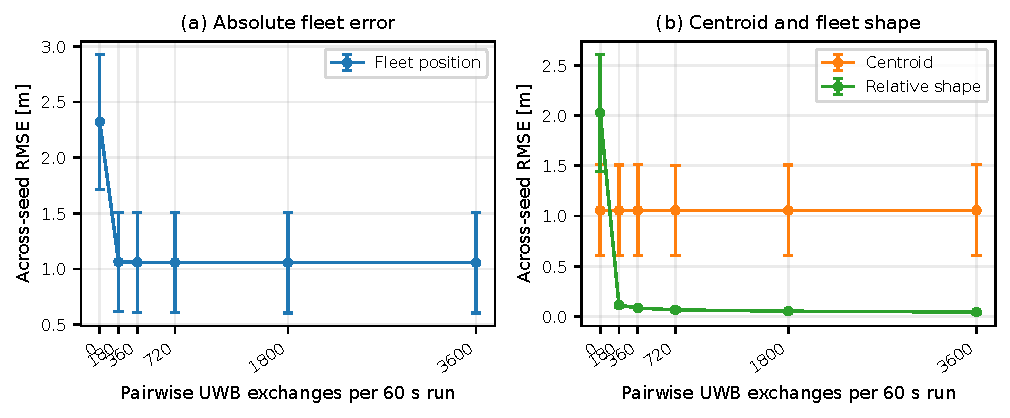
\includegraphics[width=0.98\textwidth]{figures/phase2/p2b_rate_sweep.pdf}
    \caption{P2B empirical accuracy--communication curve. Each marker shows the mean whole-run RMSE across 20 matched seeds; error bars show one sample standard deviation across seeds. (a) Absolute fleet position error. (b) Fleet-centroid error and centered relative-shape error. The horizontal axis counts pairwise UWB exchanges per \SI{60}{s} run. The two error components are displayed as separate across-seed RMSE means, not additive quantities.}
    \label{fig:p2b_rate_sweep}
\end{figure}

\subsection{Time-domain behavior and decision}
Figure~\ref{fig:p2b_time_profiles} shows instantaneous fleet RMS, centroid, and shape RMS error at selected rates. Curves are pointwise means across the 20 seeds and shading is one pointwise sample standard deviation, clipped at zero. The bands describe variability among sensor realizations, not confidence intervals for a mean trajectory. The 0 Hz shape curve is omitted from the bottom panel so that differences between the three positive rates remain legible; its divergence is shown in Fig.~\ref{fig:p2b_rate_sweep} and in the upper panel here. All four centroid trajectories nearly coincide, while the low-rate shape history has modest excursions between two-second all-link rounds.

\begin{figure}[htbp]
    \centering
    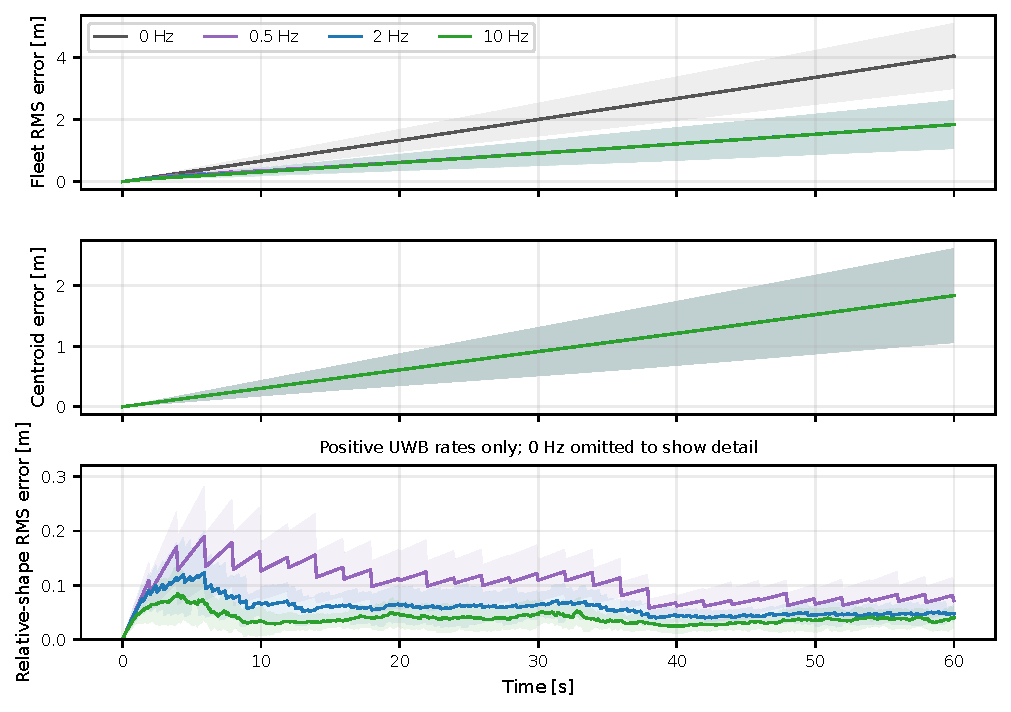
\includegraphics[width=0.98\textwidth]{figures/phase2/p2b_time_profiles.pdf}
    \caption{P2B time-resolved errors for 0, 0.5, 2, and 10 Hz on 20 matched seeds. Means and one sample-standard-deviation bands are evaluated separately at each time instant. The shape panel omits the IMU-only curve and uses a close vertical scale to distinguish the positive-rate schedules.}
    \label{fig:p2b_time_profiles}
\end{figure}

On the sampled rates, \SI{0.5}{Hz} already captures most of the achievable absolute fleet-RMSE reduction because the remaining error is dominated by common translation. Further ranging buys smaller but consistent improvements in fleet shape and worst-node error. This observation is specific to the frozen paths, IMU model, initial-pose knowledge, and idealized Gaussian ranges. It does not identify the minimum useful rate below \SI{0.5}{Hz}, nor does exchange count represent actual radio energy.

The P2B result supplies the uniform all-pairs reference for \textbf{P2C}. At matched budgets such as 180, 360, and 720 exchanges, P2C will test whether choosing different links and times can improve fleet and worst-node accuracy or fleet shape. The infrastructure-free centroid limitation remains part of that comparison rather than being hidden by the absolute fleet-RMSE plateau.
